\q{Vérifier expérimentalement que le temps de calcul du tri rapide est
  proportionnel à $n log(n)$ pour $n\in [200, 500, 1000, 5000, 10000, 100000]$}\\

Imports
\codeFromFileT{main.py}{section-01/q6/1.py}
\il{traceTemps}
\codeFromFileT{main.py}{section-01/q6/2.py}
Je le teste, mais pour \il{n = 10000}, il y a une erreur python :
on a fait trop de tour de boucle récursive...
\codeFromFileT{main.py}{section-01/q6/3.py}
Et j'obtiens :
\begin{center}
  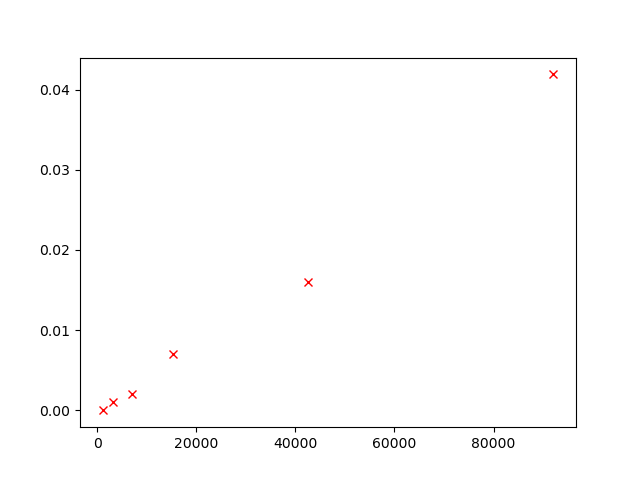
\includegraphics[scale=0.5]{section-01/q6/4.png}
\end{center}
C'est presque une droite, ce qui prouve expérimentalement la comlexité en
$n\cdot log(n)$.
